\section{Software Development Approach}

\subsection{Choice of Development Approach and Rationale}

The group has decided to follow an agile development methodology throughout the software development stage. According to~\cite{book:software_engineering_economics}, the cost of removing a software defect or implementing substantial change rises exponentially for each stage of the development cycle when it remains undiscovered. Consequently, the group must start considering the best way to effectively handle inevitable change throughout the project’s lifecycle. If the group opted to combat this change by following the traditional waterfall approach and anticipating the complete set of requirements early on then it could quickly be accused of being unresponsive to changing business conditions. \cite{art:agile_business_innovation} assert that a much better strategy can be espoused from the agile method, in which the group can attempt to reduce the cost of change throughout the project by:

\begin{itemize}
  \item Producing weekly deliveries in order to achieve an early win and acquire rapid feedback
  \item Inventing simple solutions, so there is less to change and making those changes is easier
  \item Testing constantly in an automated manner, for earlier, less expensive, defect detection
\end{itemize}

\cite{art:adaptive_sdpm} assert that the main disadvantages of agile models are poor quality product, poor design and improper documentation. Fortunately, the group can effectively tackle the abovementioned issues in the following manner: disciplined sprint cycles, version control, automated unit testing, test/behaviour driven development, continuous integration, and adequate team structure.

\subsection{Sprint Cycle}

\begin{figure}
  \centering
  \begin{minipage}{10cm}
    \centering
    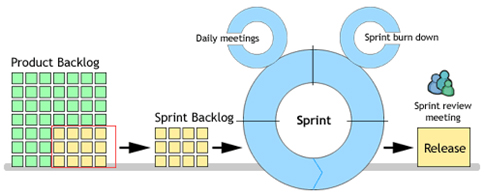
\includegraphics[width=10cm]{inc/sprint_cycle.jpg}
    \caption{Sprint Cycle}
    \label{fig:spint_cycle}
  \end{minipage}
\end{figure}

A sprint is \emph{``a regular, repeatable work cycle in scrum methodology during which work is completed and made ready for review''}~\parencite{web:scrum_sprint}. It is a core part of the agile approach and will see the group working to \~1 week sprints over a 10 week period, consequently completing \~10 sprints throughout the duration of the project. In addition, it will generate a sense of accountability and ownership within the group, as it promotes transparency, frequent review and constructive discussion.

Software requirements identified at the outset of the project will be maintained in a product backlog, where they are prioritised by business value~\parencite{book:agile_excellence}. The group will receive feedback on which items to prioritise after discussions with the target audience who have a vested interest in the product. Prior to commencing a sprint, the group will have a sprint planning meeting. During this meeting, the group will decide which items to add to the sprint, and identify the tasks necessary to complete each item. If possible, the group will estimate how many hours each task will take someone to complete~\parencite{web:scrum_sprint}. As team engagement and morale is likely to fluctuate from sprint to sprint, it will be important to get verbal approval from everyone about the commitments being made at the time.

The sprint will commence immediately after the planning meeting. Throughout the sprint, the group will have daily meetings (Monday to Friday and excluding public holidays) on the WhatsApp messaging platform or face-to-face if possible. During this meeting, everyone will be asked:

\begin{itemize}
  \item What did you do yesterday?
  \item What are you doing today?
  \item Are there any currently impediments in your way?
\end{itemize}

At the end of each sprint, the group will have a sprint review meeting. During this meeting, the group will show what they have accomplished during the sprint and demo any newly added features. In addition, the current state of the project is assessed against the goal determined during the sprint planning meeting. Ideally, the team would have completed each product backlog item bought into the sprint, but if they have not then the item will be carried over into the next sprint~\parencite{web:scrum_sprint}.

\subsection{Version Control}

\begin{figure}
  \centering
  \begin{minipage}{10cm}
    \centering
    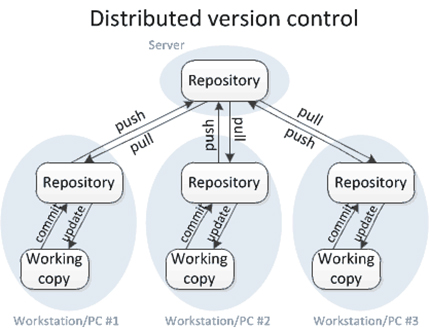
\includegraphics[width=10cm]{inc/distributed_version_control.jpg}
    \caption{Distributed Version Control}
    \label{fig:distributed_version_control}
  \end{minipage}
\end{figure}

Version control is \emph{``a system that records changes to a file or set of files over time so that you can recall specific versions later''}. Consequently, a version control system will allow the group to revert files to a previous state, compare changes over time, and see who last modified something that might be causing a problem~\parencite{web:git}. The group will be using GitHub, a distributed version control system. As a result, each group member will need to commit their changes to local repository on their computer before pushing them to a server, instead of directly checking them into the server repository~\parencite{book:pro_tfs}. By splitting up the process into two steps, group members can carry out the necessary due diligence to ensure that their code does not break the solution by testing their changes locally.

\subsection{Automated Unit Testing}

\begin{figure}
  \centering
  \begin{minipage}{7cm}
    \centering
    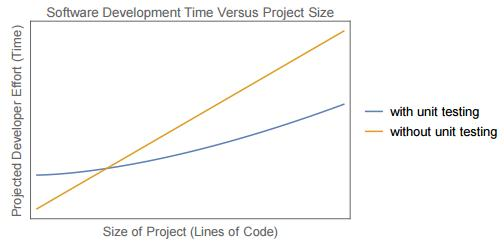
\includegraphics[width=10cm]{inc/automated_unit_testing.jpg}
    \caption{Development Time for a Software Project}
    \label{fig:automated_unit_testing}
  \end{minipage}
\end{figure}

According to Sharma, et al~\parencite{rep:unit_testing_validation}, a unit test is a function that compares an input-output pair and then returns a Boolean value. A result of True indicates that he code is behaving as intended, but a result of False indicates that it is not, and consequently, that any program relying on that code cannot be trusted to have as intended. To reduce the overall development time, the group will need to create unit tests in order to reduce the number of errors in the application. A well designed unit tests will allow the group to make sweeping changes to the code quickly, as everyone will better understand the design of the code being worked on. This will be helpful when the group starts to document the solution, as it will be easier to define what each part of the application is supposed to do.

\subsection{Test/Behaviour Driven Development}

\begin{figure}
  \centering
  \begin{minipage}{7cm}
    \centering
    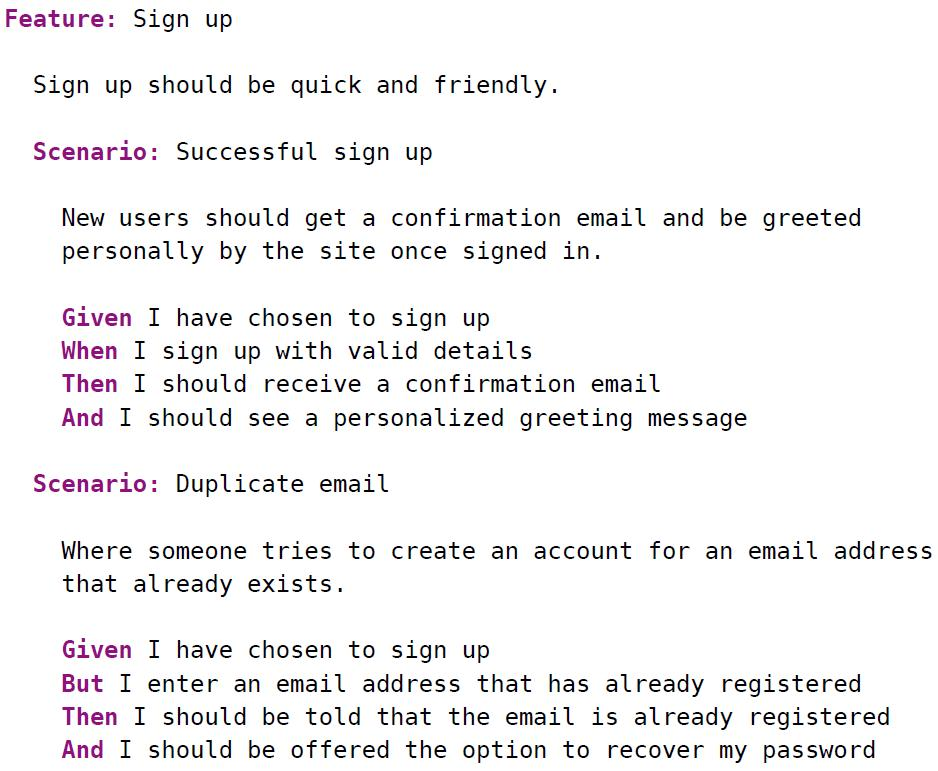
\includegraphics[width=7cm]{inc/behaviour_driven_development.jpg}
    \caption{Behaviour-Driven Development}
    \label{fig:behaviour_driven_development}
  \end{minipage}
\end{figure}

The group will not write unit tests after all of the software is written. Instead, each unit test will be written beforehand in order to reduce the likelihood of producing bad code -- employing a test-driven development (TDD) approach which involves the following steps as suggested by~\cite{book:art_of_unit_testing}:

\begin{itemize}
  \item Write a failing test to prove code or functionality is missing from the solution. For example, if a group member wanted to add a new feature to the solution that remembers the user’s age, then they would need to write a test that verifies that the age is indeed a number. At this point, the test should not pass because the solution currently lacks that functionality.
  \item Make the test pass by writing code that meets the expectations of the test.
  \item Refactor the code to ensure that a piece of code is easier to read and maintain, while still passing all of the previously written tests.
\end{itemize}

Alternatively, the group can also experiment with a behaviour-driven development (BDD) approach, in which the intent of the system is tested. This is different to the TDD approach, as the group will be focused on writing scenarios that prove code or functionality is missing from the solution by writing a failing customer acceptance test that describes the behaviour of the system from the customer's point of view~\parencite{book:art_of_unit_testing}. A scenario must be written in manner that can easily be read or written by any group member. North~\parencite{web:behaviour_driven_development} affirms that this can done by using a common vocabulary that spans the divide between business and technology. As a result, it become a communication and collaboration tool. Consequently, business stakeholders can be drawn into the software development process, helping the group better understand their requirements~\parencite{web:behaviour_driven_development}.

\subsection{Continuous Integration}

\begin{figure}
  \centering
  \begin{minipage}{7cm}
    \centering
    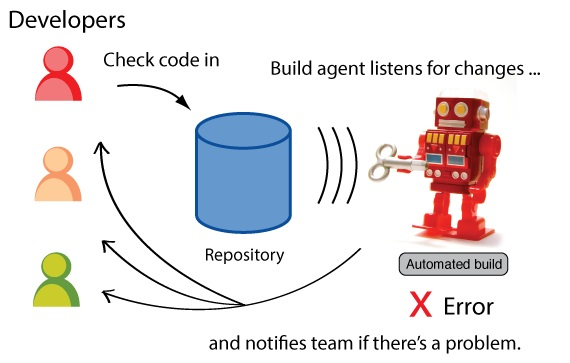
\includegraphics[width=7cm]{inc/continuous_integration_process.jpg}
    \caption{Continuous Integration Process}
    \label{fig:continuous_integration_process}
  \end{minipage}
\end{figure}

Continuous integration (CI) is a software development practice in which updates to the solution are immediately tested and reported on when they are added to the main codebase. In using CI, the group will receive rapid feedback so that if a defect is introduced, it can be identified and corrected as soon as possible~\parencite{web:behaviour_driven_development}. The group will be using Travis CI, an open-source continuous integration service to automatically build and test the solution hosted at GitHub. According to~\cite{book:ci_NET}, if the group implements and maintains relatively good CI processes, they are more likely to create a better solution, as they would have done testing and integration consistently earlier in the process, reducing the chances of catching bugs later. Furthermore it promotes transparency, as each group member will be able to see the results of the build and know where the problems are.

\subsection{Team Structure}

The group is comprised of ``generalising specialists'' -- individuals who have one or more technical speciality coupled with general knowledge of the business domain, so they can deliver direct value to the project in a numerous ways and easily change roles if required at a later stage. Furthermore, as a changing group structure is detrimental to achieving any set objectives, it is expected that the group will remain as stable throughout the course of the project~\parencite{book:agile_development}.
